\chapter{背景と目的}\label{chap:background}

%%%%%%%%%%%%%%%%%%%%%%%%%%%%%%%%%%%%%%
%      業界の背景
%        - 注目
%        - 同期編集とは?
%        - メリット
%        - 課題点
%%%%%%%%%%%%%%%%%%%%%%%%%%%%%%%%%%%%%%
\section{背景}
近年, Googleドキュメント\cite{GOOGLEDOCS}やMicrosoft Word Online\cite{WORDONLINE}に代表されるテキスト編集を中心に, 同期編集システムの研究や開発が注目されている.
同期編集とは, 複数人で同一のデータを同時に編集できるシステムである.
複数人で行うため, 作業効率が上がることや, 他の人が作っている部分を見ながら自分の作業している部分を修正できるメリットがある.
また, 個々で作られたファイルをマージする手間も削減できる.
同期編集では, 複数のユーザから様々な編集が行われ, あるユーザが最新ではないデータを編集する際に, 編集の衝突が起こる. 衝突が起こると各ユーザが扱うデータに矛盾が生じ, データの同期が失敗する可能性がある. データに矛盾が生じる例を図\ref{mujyun}に示す.
こういった衝突を解消することが同期編集の主な課題となっている.
衝突を解消するための同期機構にはいくつか選択肢があり, 後で変更することは困難となるのでアプリケーションの開発サイクルの早い段階で選択する必要がある.
\begin{figure}[htbp]
  \begin{center}
    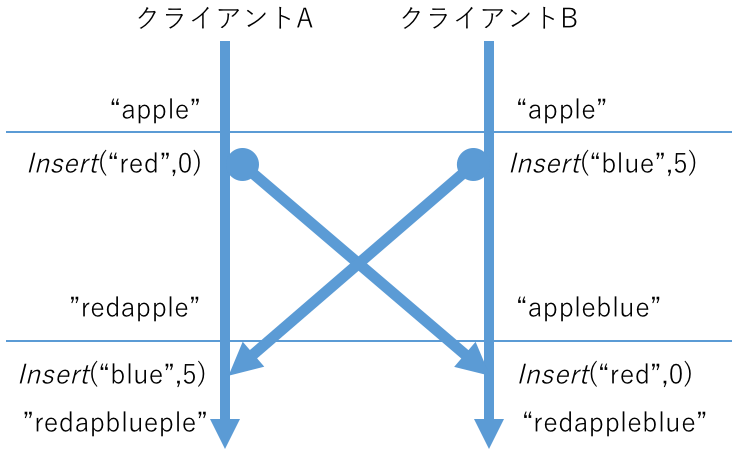
\includegraphics[scale=0.3]{images/mujyun}
    \caption{矛盾が生じる例}
    \label{mujyun}
  \end{center}
\end{figure}
\par
また, 3Dモデリングで扱う頂点や面などの, 3次元データを扱う同期編集システムも研究や開発が行われている. 3次元データを扱う際, 例えば, 面と頂点のデータ間にある依存関係を考慮しなければならない. 現在の研究では, オブジェクト単位の同期と, 依存関係のないデータのみの同期編集に留まっている. より柔軟に同期編集をするには, 依存関係を考慮し, 頂点の操作も含めた3次元データの同期する必要がある.

%%%%%%%%%%%%%%%%%%%%%%%%%%%%%%%%%%%%%%
%      関連研究
%       - OT
%       - three-way merges
%       - Differential Synchronization
%       - CoMaya
%       - WFE/threesession
%%%%%%%%%%%%%%%%%%%%%%%%%%%%%%%%%%%%%%
\section{関連研究}
%
\subsection{Edit-based}
Edit-basedは, ユーザの全ての操作を他のユーザに反映させる同期機構である.
アルゴリズムとして操作変換(Operation Transformation : OT)\cite{OT}を扱う.
操作変換は, ある編集操作のデータを, 以前に実行された編集操作の結果によって更新する仕組みである.
これにより, 編集の衝突によるデータの矛盾を防ぐことができる.
図\ref{ot}は図\ref{mujyun}の矛盾を操作変換を用いて解消した例である.
\begin{figure}[htbp]
  \begin{center}
    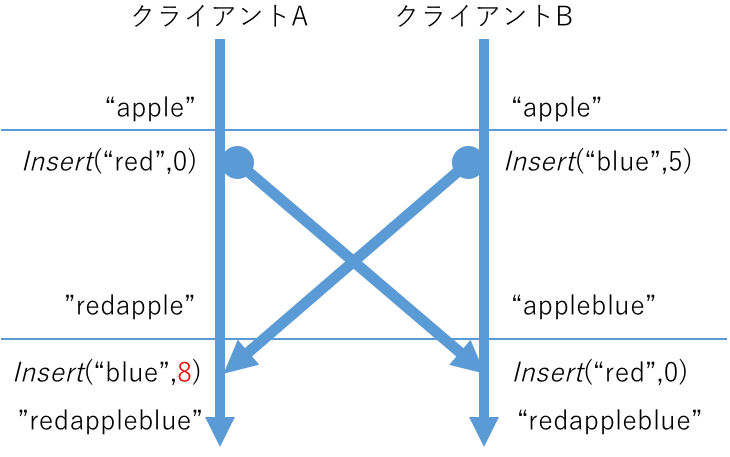
\includegraphics[scale=0.3]{images/ot}
    \caption{操作変換}
    \label{ot}
  \end{center}
\end{figure}
%
\subsection{three-way merges}
three-way mergesはあるユーザの編集と, そのユーザ以外のユーザによる編集と, ベースとなる元ファイルの3つのデータを, サーバでマージし最新のファイルを作る. その最新のファイルをユーザに送信し, 同期を行う同期機構である. ベースとなる元ファイルの存在により, ユーザによる最新ではないデータに対する編集があっても, データの矛盾は生じない.
three-way mergesの流れの概略図を図\ref{threeway}に示す.
\begin{figure}[htbp]
  \begin{center}
    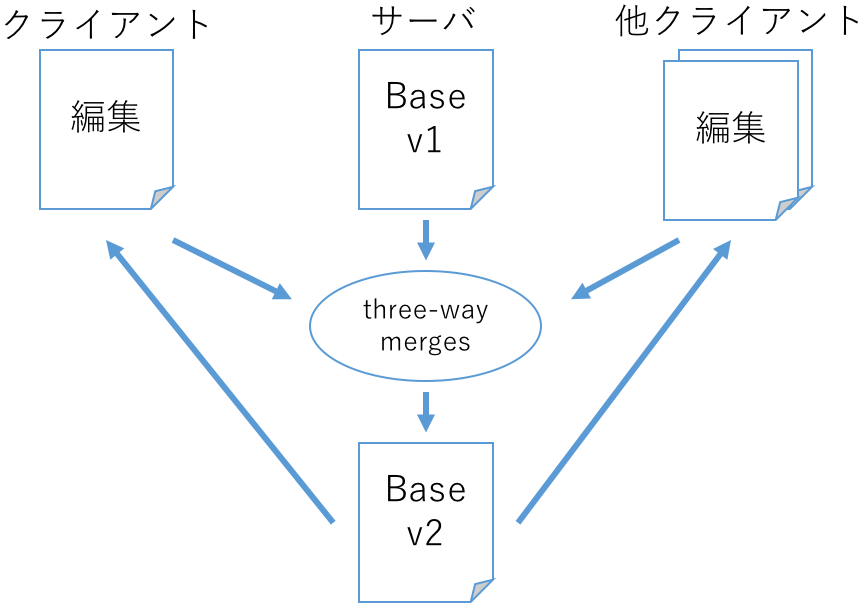
\includegraphics[scale=0.3]{images/threeway}
    \caption{three-way merges}
    \label{threeway}
  \end{center}
\end{figure}
%
\subsection{Differential Synchronization}
Differential Synchronization\cite{DS}は差分の計算とその適用によって同期を行う. 図\ref{DSfig}はDifferential SynchronizationのDual Shadow Methodの同期の流れである.
\begin{figure}[htbp]
  \begin{center}
    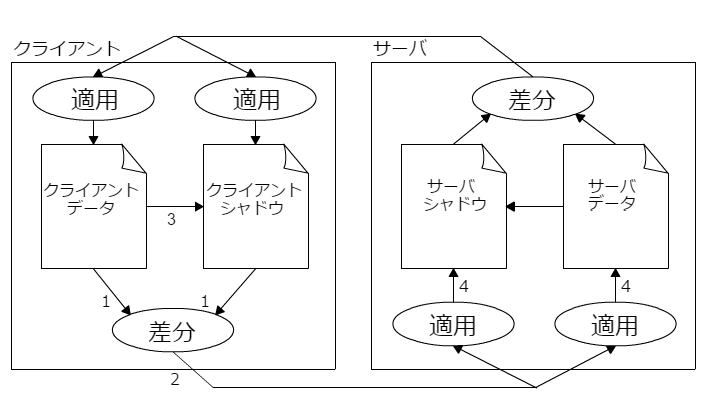
\includegraphics[scale=0.7]{images/DS}
    \caption{Differential Synchronization}
    \label{DSfig}
  \end{center}
\end{figure}
Dual Shadow Methodは, クライアントデータとサーバデータの他に, クライアントとサーバに各データのシャドウコピーを用意する. 処理の流れとしては, まずクライアントデータとそのシャドウの差分を計算しサーバに送信する. 次に, サーバで適用処理を行い, クライアントではシャドウコピーを行う. サーバ側でも同様の手順で行うことで同期が可能となる. サーバデータは複数クライアントから利用され, クライアントデータと2つのシャドウは接続しているクライアントごとに用意される. 2つのシャドウコピーは各適用処理の後, 必ず一致する仕組みになっている. 編集が衝突し, データに矛盾が生まれた場合でも, それぞれ差を計算し適用することによって各データが同一のものに収束する.
%
\subsection{CoMaya}
CoMaya\cite{COMAYA}は3D統合ソフトMayaのAPIを利用し, 3Dモデリングにおける同期編集を可能にしたものである. オブジェクトのデータとMayaのAPIを一次元に管理して, 操作変換を適用して同期を行なっている. そのため, オブジェクトと面や, 面と頂点間の依存関係を解決できておらず, オブジェクトの位置やマテリアルの同期に留まっている.
%
\subsection{WFE}
WFE\cite{WFE}はWebページの同期編集を可能にしたシステムである. ある時点でのサーバデータにおけるスナップショットと各ユーザによる編集データを用い, three-way mergesに似た同期機構を採用している. WebページのHTMLにおけるDOM要素を編集単位として同期を行なった.
%%%%%%%%%%%%%%%%%%%%%%%%%%%%%%%%%%%%%%
%      threesession
%%%%%%%%%%%%%%%%%%%%%%%%%%%%%%%%%%%%%%
\section{3次元データのthree-way mergesへの適用}
WFEを参考に3次元データのthree-way mergesへの適用を試みた.
システムは, 頂点編集が可能なクライアントと、編集のデータを管理するサーバプログラムによって構成した. ユーザの操作ごとにクライアントが編集のデータをサーバに送信し, サーバはその時点でのスナップショットと各ユーザの編集をマージした. クライアントは一定時間ごとにデータをサーバから受信し適用した. これらの手順よりクライアント間でデータの同期を行なった. 各ユーザのデータは一致し同期可能であった. しかし, スナップショットをポーリングにより取得するため, 頂点が増えデータの容量が増大する可能性がある3次元データでは対応しきれない.
%%%%%%%%%%%%%%%%%%%%%%%%%%%%%%%%%%%%%%
%      自分の研究の目的
%%%%%%%%%%%%%%%%%%%%%%%%%%%%%%%%%%%%%%
\section{目的}
本研究では, 依存関係の扱いが操作変換より容易になり, 送受信の容量が少なくて済むと予想されるDifferential Synchronizationの同期手法に基づいて, 3次元データの依存関係を考慮した同期編集機構の手法を提案する.
これにより, 複数人で同一の3次元データを同時に編集できる3Dモデリングソフトの開発を可能にする.
